% Paper template for TAR 2018
% (C) 2014 Jan Šnajder, Goran Glavaš, Domagoj Alagić, Mladen Karan
% TakeLab, FER

\documentclass[10pt, a4paper]{article}

\usepackage{tar2018}

\usepackage[utf8]{inputenc}
\usepackage[pdftex]{graphicx}
\usepackage{booktabs}
\usepackage{amsmath}
\usepackage{amssymb}
\usepackage{algorithm}
\usepackage[noend]{algpseudocode}

\title{Hate Speech Identification Using Active Learning}

\name{Stjepanović Mateo, Žabčić Mislav, Tolić Filip} 

\address{
	University of Zagreb, Faculty of Electrical Engineering and Computing\\
	Unska 3, 10000 Zagreb, Croatia\\ 
	\texttt{\{mateo.stjepanovic, mislav.zabcic, filip.tolic\}@fer.hr}\\
}


\abstract{ 
	In this paper, we tackle the problem of detecting hate speech and finding a difference between hate speech and offensive language. We know that some machine learning approaches got good results when distinguishing the hate speech from offensive language. Problem with almost all machine learning approaches is that we need a lot of data to train model well. The main idea of this work is not to fix the results of previous machine learning methods, or to outperform them, but to get similar results with much less data on which model can learn. Our results show that using even baseline semi-supervised active learning model can reduce data we need to learn model on the same level.
}

\begin{document}
	
	\maketitleabstract
	
	\section{Introduction}
	\begin{table*}[t!]
		\centering
		\resizebox{\textwidth}{!}{%
			\begin{tabular}{lll}
				&                       &                                                                                                                             \\ \hline
				\multicolumn{1}{l}{Tweets before cleaning} & \multicolumn{1}{l}{} & \multicolumn{1}{l}{Lmao RT @MoeMartin44 The in soles in Reebok Classics can't even handle diabetic weight Rick Ross holds} \\ \hline
				\multicolumn{1}{c}{Array of words}         & \multicolumn{1}{l}{} & \multicolumn{1}{l}{lmao, sole, reebok, classic, can't,  even, handl,  diabet, weight, rick,  ross, hold}                   \\ \hline
			\end{tabular}%
		}
		\caption{First row shows the original tweet post from the dataset, the second row shows cleaned, tokenized and stemmed tweet post}
		\label{tbl:prepData}
	\end{table*}
	
	The impact that social media have on our daily lives has kept growing for the last 15 years. With the appearances of social media like Twitter, Facebook, Tumblr and many others, interactions between the users and the ability to express their opinions have never been easier. The rise in the use of hate speech, incited by the evolution of social media, was followed by the need to detect it. Facebook CEO, Mark Zuckerberg, predicts that in a 5 to 10 year period they will have the AI tools necessary to build a successful hate speech detection machine. What makes the detection of hate speech such a difficult task? To address that question we have to define hate speech. We define hate speech as communication that expresses hate towards a certain group of people based on their race, ethnicity, national origin, gender, religion, sexual orientation, etc. It often includes the use of offensive language or cuss words. It is important to differ offensive language from hate speech because people often use offensive language in their everyday language. Most rap songs, which people often cite, are filled with offensive words such as b*tch, n*gga, wh*re, etc. While communicating with their closest friends, people often use cuss words as a joke with no intention of hurting the other person. Because of situations like these, we need to build a classifier that recognizes the difference between hate speech and offensive language. 
	
	\begin{figure}[h]
		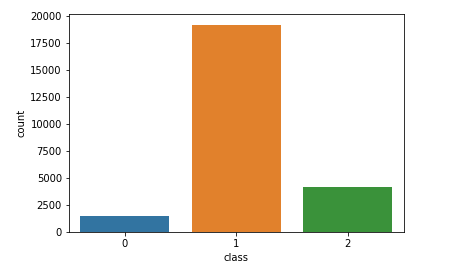
\includegraphics[width=1.1\linewidth, height=0.25\textheight]{pictures/HistOfData}
		\caption[Histogram showing number of labeled classes]{Histogram shows the imbalanced dataset. Tweets from dataset were extracted using \textit{hate} words from Hatebase but not many of them contained hate speech. Drawn using \citep{Matplotlib,seaborn}}
		\label{fig:histofdata}
	\end{figure}
	
	We use the dataset annotated by CrowdFlower workers. The workers were asked to annotate 25000 tweets into 3 categories: hate speech (class 0), offensive language (class 1) and speech that contains neither hate speech nor offensive language (class 2). A clear imbalance in the dataset is shown in a histogram displayed in Figure \ref{fig:histofdata}.\citet{Davidson2017AutomatedHS} used logistic regression to detect hate speech. Even though their model was rather successful, they still struggled with separating hate speech from offensive language. In this paper, we explore the use of active learning to deal with the problems of separating offensive language from hate speech and solving the imbalance of the used dataset.
	
	
	\section{Related work}
	
	Hate speech is a big, unresolved problem in the modern-day society. Even companies as big as Facebook are still struggling with it. It is important to separate hate speech from offensive language, even so, because of new laws against hate speech\citep{Davidson2017AutomatedHS}. As said in \citet{Davidson2017AutomatedHS} offensive language is mostly used in everyday life and often does not do any harm. Authors in that same paper tried few variants of models and decided that Logistic Regression with L2 regularization is the best model right now.
	While this problem is yet to be solved there is no discovered set of features that surely works. In \citet{Davidson2017AutomatedHS} they used several features to capture information about syntactic and semantic structures. Porter stammer is used to create unigram, bigram and trigram features and then used TF-IDF to put weights to them. Using NLTK library they constructed Part of Speech tags as features. They showed that their model is working great, and got pretty high official metrics (precision, recall and average F1 score). In the introduction to their paper, they stated that lexical structures often mislead model and produces false positives on hate speech. \citep{Davidson2017AutomatedHS}
	\\\citet{WaseemUnderstandingAbuse} stated and gave an example of one reason why today we cannot get relevant scores or datasets. As the stated problem is that there is no consensus on what falls under what category. So they proposed a new separation method. It consists out of two questions \citep{WaseemUnderstandingAbuse}:
	\begin{itemize}
		\item \textit{Is the language directed towards a specific individual or entity or is it directed towards a generalized group?}
		\item \textit{Is the abusive content explicit or implicit?}
	\end{itemize}
	Answering those questions we can differ between four main classes:
	\begin{itemize}
		\item \textit{Directed Implicit}
		\item \textit{Generalized Implicit}
		\item \textit{Directed Explicit}
		\item \textit{Generalized Explicit}
	\end{itemize}
	
	\\\citet{ChenSVMFeatures} shows that one can implement feature selection methods into SVM itself\citep{ChenSVMFeatures}. This could possibly enable great future work in trying to achieve an end-to-end solution for the hate speech identification problem, as we encountered the problem of a high number of features, and high CPU and RAM requirement as result of that. In our paper, we used baseline features because we did not want to focus ourselves on feature selection. The approach proposed by \citet{ChenSVMFeatures} gives us an idea of how to improve our model later on.
	\\The problem of data size and time needed to manually label data was always been in machine learning. That is why active learning as the semi-supervised approach is developed. \citet{LuoALPlankton} proposed a new active learning model based on multi-class support vector machines. They showed that there is a way to make SVM work with probabilities and give us a proper active learning model. Even though we did not implement this model, the plan is to implement it in the future and test it on state-of-the-art models. Their algorithm works as follows\citep{LuoALPlankton}:
	\begin{itemize}
		\item 1. Start with an initial training set and an unclassified set.
		\item 2. A multi-class support vector machine is built using the current training set.
		\item 3. Compute the probabilistic outputs of the classification results for each data on the unclassified set. Suppose the class with the highest probability is a and the class with second highest probability is b. Record the value of P(a) and P(b) for each unclassified data.
		\item 4. Remove the data from the unclassified set that has the smallest difference in probabilities between them (P(a) − P(b)) for the two highest probability classes, obtain the correct label from human experts and add the labeled data to the current training set.
		\item 5. Go to 2
	\end{itemize}
	\\\citet{YangMultiClassAL} introduced their own active learning model based on multi-class SVMs. It is a little different from one before on manner that they calculate probability on each data in the unlabeled pool. Considering that, their model is computationally expensive if unlabeled pool in large size\citep{YangMultiClassAL}. Their experiment also shows that they outperform state-of-the-art models, which can only be a sign to continue further on our work to create an end-to-end solution for hate speech identification.
	\section{Preparing data}
	\begin{table*}[t!]
		\centering
		\caption{Table shows how precision, recall and F1 score behaves on different iterations.}
		\label{tbl:Scores}
		\begin{tabular}{lllllllllllllllll}
			\hline
			& Iteration             & \multicolumn{3}{c}{0}                                                             &                       & \multicolumn{3}{c}{40}                                                            &                       & \multicolumn{4}{c}{60}                                                                                    & \multicolumn{3}{c}{100} \\ \hline
			\multicolumn{1}{l}{}  & \multicolumn{1}{l}{} & \multicolumn{1}{l}{P}    & \multicolumn{1}{l}{R}    & \multicolumn{1}{l}{F1}   & \multicolumn{1}{l}{} & \multicolumn{1}{l}{P}    & \multicolumn{1}{l}{R}    & \multicolumn{1}{l}{F1}   & \multicolumn{1}{l}{} & \multicolumn{1}{l}{P}    & \multicolumn{1}{l}{R}    & \multicolumn{1}{l}{F1}   & \multicolumn{1}{l}{} & P      & R      & F1     \\ \hline
			\multicolumn{1}{l}{Class 0} & \multicolumn{1}{l}{} & \multicolumn{1}{l}{0.11} & \multicolumn{1}{l}{0.04} & \multicolumn{1}{l}{0.06} & \multicolumn{1}{l}{} & \multicolumn{1}{l}{0.23} & \multicolumn{1}{l}{0.13} & \multicolumn{1}{l}{0.17} & \multicolumn{1}{l}{} & \multicolumn{1}{l}{0.35} & \multicolumn{1}{l}{0.20} & \multicolumn{1}{l}{0.25} & \multicolumn{1}{l}{} & 0.37   & 0.19   & 0.25   \\ \hline
			\multicolumn{1}{l}{Class 1} & \multicolumn{1}{l}{} & \multicolumn{1}{l}{0.80} & \multicolumn{1}{l}{0.91} & \multicolumn{1}{l}{0.85} & \multicolumn{1}{l}{} & \multicolumn{1}{l}{0.82} & \multicolumn{1}{l}{0.90} & \multicolumn{1}{l}{0.86} & \multicolumn{1}{l}{} & \multicolumn{1}{l}{0.82} & \multicolumn{1}{l}{0.91} & \multicolumn{1}{l}{0.86} & \multicolumn{1}{l}{} & 0.82   & 0.91   & 0.86   \\ \hline
			\multicolumn{1}{l}{Class 2} & \multicolumn{1}{l}{} & \multicolumn{1}{l}{0.47} & \multicolumn{1}{l}{0.30} & \multicolumn{1}{l}{0.37} & \multicolumn{1}{l}{} & \multicolumn{1}{l}{0.52} & \multicolumn{1}{l}{0.37} & \multicolumn{1}{l}{0.43} & \multicolumn{1}{l}{} & \multicolumn{1}{l}{0.53} & \multicolumn{1}{l}{0.36} & \multicolumn{1}{l}{0.43} & \multicolumn{1}{l}{} & 0.51   & 0.36   & 0.42   \\ \hline
		\end{tabular}
	\end{table*}
	We used the dataset that was introduced in \citet{Davidson2017AutomatedHS}. They prepared the data by annotating the twitter posts with three available classes: 0 meaning it is a hate speech, 1 being an offensive language and 2 being nothing of previous two. People from CrowdFlower annotated the data by marking each tweet, they classified the tweet by majority class. The minimum number of annotators for each tweet was three.
	As seen in Figure \ref{fig:histofdata} data is unevenly distributed. That has a big influence on learning outcomes. We used traditional NLP methods to prepare the data.
	\\First, we had to clear the text from all of the usual twitter "stuff", like hashtag or mentions. To remove these certain things, we use regular expressions to automate the process. Together with hashtags and mentions, we removed URL, times, dates.
	\\After clearing the text, we switched it to lower case and converted it to tokens. These tokens were stemmed using Porter stemmer \citep{PorterStemmer}.
	\\Using \textit{NLTK} library \citep{NLTK} we removed all classical stop words in the English language. After tokenization, 50 of the most frequent words are removed (same as removing dataset specific stopwords), that allowed us to lower the number of our features. That same size was one of the biggest problems in our work.
	We tried doing that on our baselines and got much better results so we used that approach to active learning.
	\\The last thing we had to do is to turn these tokens into a vector. We used TF-IDF vectorizer, from the \textit{sklearn} library \citep{scikit-learn}, to extract features from our text. After testing the removal of said words, we got considerably better results on our baseline models so we used the same approach in our active learning based model.
	After using all these methods, we were ready to train our baseline and our active learning models
	
	Table \ref{tbl:prepData} shows the output of our data preparation. After text cleaning, tokenization and so on, we got an array of words that represents the input tweet from the dataset.
	
	\section{Model Overview}
	As stated above, one of the biggest problems is that we need a lot of annotated to train model properly. This problem presents itself in the hate speech identification as there is no relevant or good enough database. Database introduced in \citet{Davidson2017AutomatedHS} suffers from the lack of equal distribution of data across all three classes. To sidestep that problem, we decided to go with a semi-supervised model. A model whose training is based on, so-called, active learning.
	\\While this is just a brief overview and some kind of prototype to show us if active learning is a good approach, we introduced just one of the baseline models for active learning. Label Spreading and Label Propagation are the only two semi-supervised model that one can find in the \textit{sklearn} library \citep{scikit-learn}.
	\\\citet{LuoALPlankton} and \citet{YangMultiClassAL}, it is shown that active learning can be of much use when it comes to the problem of too few data.
	\\The main idea of active learning is that in the first step we take a small subset out of the training set and train our model on it. In the next step, we need to calculate the  probabilities of a good estimation of the model for the remaining training set. Given these probabilities, we then choose a subset of that data that has the lowest probability of estimation. After that model is trained on the calculated set. We repeat the previous steps until we either reach the maximum number of iterations or gain satisfactory results.
	The active learning algorithm can be summed in three steps:
	\begin{itemize}
		\item \textit{1. Select m size subset from the training set}
		\item \textit{2. Train label spreading model on given subset}
		\item \textit{3. Predict probabilities on the remaining training set}
		\item \textit{4. Select n worst probabilities and  use that data to expand the initial training set}
		\item \textit{5. Go to 2.}
	\end{itemize}
	\\In our work, we set the maximum number of iterations and training subset size to $100$. These numbers were chosen to better capture the peak point of the algorithm. If we chose too big of a number, we could not accurately determine when did the model reach optimal results. On the other hand, if we chose too small of a number, training a model on a such a small subset would not make much sense. With these hyperparameters, we got the desired results after half of the maximum iterations, and we kept running the other half to see how the model will behave.
	
	
	
	Table \ref{tbl:Scores} show how are metric improved through time.
	In table \ref{tbl:Scores} we can see that the optimal results are achieved after only 60 iterations. That is about $6000$ labeled data on which we train our model.
	
	In next section, it is shown that our model, based on active learning, even though it is baseline model, has a lot of potential for future work.
	\begin{table*}[t!]
		\centering
		\caption{Table shows average F1 scores for every class individually and micro averaged F1 for all classes together for each of our models. It also contains estimated average time needed to train one of ten K folds in our cross-validation.}
		\label{tbl:scoreOur}
		\begin{tabular}{lccccc}
			\hline
			& \multicolumn{1}{l}{F1(hate)} & \multicolumn{1}{l}{F1(offensive)} & \multicolumn{1}{l}{F1(clean text)} & \multicolumn{1}{l}{F1(all)} & \multicolumn{1}{l}{Training time(minutes)} \\ \hline
			Logistic Regression                 & \textbf{0.26}                & \textbf{0.92}                     & \textbf{0.70}                      & \textbf{0.85}               & \textbf{6 min}                             \\ \hline
			\multicolumn{1}{c}{SVM}             & \textbf{0.26}                & 0.90                              & 0.55                               & 0.80                        & 70 min                                     \\ \hline
			\multicolumn{1}{c}{Active Learning} & \textbf{0.26}                & 0.87                              & 0.46                               & 0.77                        & 16 min                                     \\ \hline
		\end{tabular}
	\end{table*}
	\section{Experiments}
	We compare our active learning model to the model created by \citet{Davidson2017AutomatedHS} and two different baseline models using the same features as our model. One of those models is a logistic regression and the other is an SVM. SVM and Logistic regression were evaluated using nested cross-validation while our active learning model was evaluated on a regular cross-validation. For SVM and Logistic regression \textit{C} and \textit{gamma} were optimized as hyperparameters. Nested cross-validation used 10 outer and 5 inner folds. For our results, we use those that gave us the highest F1 score for hate speech class. The results are shown in Table \ref{tbl:scoreAll}. \citet{Davidson2017AutomatedHS} model was trained using 10000 TF-IDF features including POS tags and some general information features as tweet length, number of words, etc. Our 3 models used only 1000 TF-IDF features. We can see that because of the lack of features the F1 scores for hate class fall significantly compared to \citet{Davidson2017AutomatedHS} but they are consistent for all 3 models. We assume the reason for this is that the sklearn implementation of TF-IDF vectorizer, used in this paper, takes only top used ngrams from the dataset and this results in a substantial loss of the hate speech class features because of the imbalanced dataset.  
	\\To fix this problem, in future work we should either try to “cherry-pick“ ngrams that show in both the hate speech class and offensive language class or use a different set of features. When comparing the F1 score for all classes \citet{Davidson2017AutomatedHS} has an F1 score of 0.9 while our best model is the logistic regression with the score of 0.85. Our SVM model has an F1 score of 0.8, which is a considerable drop compared to \citet{Davidson2017AutomatedHS}, while our active learning models F1 score is only 0.03 behind SVM. Considering that the \citet{Davidson2017AutomatedHS} was trained using a substantially larger set of features, it is expected to have better results. That is why we are going to compare our active learning model to our own implementations of SVM and logistic regression that use the same set of features. All our testing was done on an Intel(R) Core(TM) i5-7200U CPU with 16 GB of RAM. 
	\\Table \ref{tbl:scoreOur}. shows the difference in F1 scores and time needed to train each model. As we can see the logistic regression class outperforms SVM and active learning model by a large margin. Even though the F1 scores for hate speech class are the same for all three models, the biggest difference is in detecting clean text with F1 scores varying from 0.46 to 0.7. Even though the clean text class has the biggest variance between the models, the biggest impact on the total F1 score comes from the offensive language class. The reason for this is the imbalanced dataset where over 70% of the data is classified as offensive language. The result of the imbalanced dataset is that offensive language class has a considerably higher recall than precision while the other two classes have a higher precision than recall.
	\begin{table}[!ht]
		\centering
		\caption{Table contains F1 scores for four different models. Column F1(hate) shows F1 scores calculated only on hate speech class while column F1(all) scores are calculated as micro average F1 scores on all three classes.}
		\label{tbl:scoreAll}
		\begin{tabular}{ccc}
			\hline
			\multicolumn{1}{l}{} & \multicolumn{1}{l}{F1(hate)} & \multicolumn{1}{l}{F1(all)} \\ \hline
			Davidson et al.      & \textbf{0.51}                & \textbf{0.90}               \\ \hline
			Logistic Regression  & 0.26                         & 0.85                        \\ \hline
			SVM                  & 0.26                         & 0.80                        \\ \hline
			Active Learning      & 0.26                         & 0.77                        \\ \hline
		\end{tabular}
	\end{table}
	Even though our active learning model has worse results than the other two models, it is important to mention that it has the smallest differences in precision and recall for each class. Why is this the case? As we mentioned, we chose active learning model as a way to train a model on a much smaller dataset. The model was trained on around 8000 and tested on approximately 2500 tweets. Because of that, the difference in the dataset distribution was not as impactful as it was on the other two models that were trained on 20000 tweets. We believe that given a balanced dataset, all our models would perform much better, but active learning would not need as much data to train itself, which is a significant step forward.
	
	\section{Conclusion}
	In the modern-day society, hate speech is becoming a great problem, but detecting it could be considered an even greater problem. It is hard for a human to detect the difference between hate speech and offensive language, and teaching a machine to solve that problem is an interesting and an ambitious project.
	\\We know that detection methods based on lexical features lack precision when it comes to separating hate speech from offensive language or detecting hate speech when no offensive language is used. Some machine learning methods give better results and that was our point of interest that we used when we started working on this paper.
	\\We used the dataset created by \citet{Davidson2017AutomatedHS} that contains a great imbalance in the distribution of the classes. To solve this problem, we implemented a semi-supervised model based on active learning. We wanted to get the same or better results than other baseline models while training on a much smaller dataset. Our implementation of an active learning model shows promising results while being simple and using only a small set of features. In future, we would like to further explore the use of active learning with a different set of features, and creating a much more computationally expensive active learning algorithm that takes into account the whole dataset and not just the training set.
	
	\bibliographystyle{tar2018}
	\bibliography{tar2018} 
	
\end{document}